% Phase-Locked Finance Validation Panel Captions
% Publication-quality LaTeX figure environments (300 DPI, white background)

\begin{figure*}[!htbp]
    \centering
    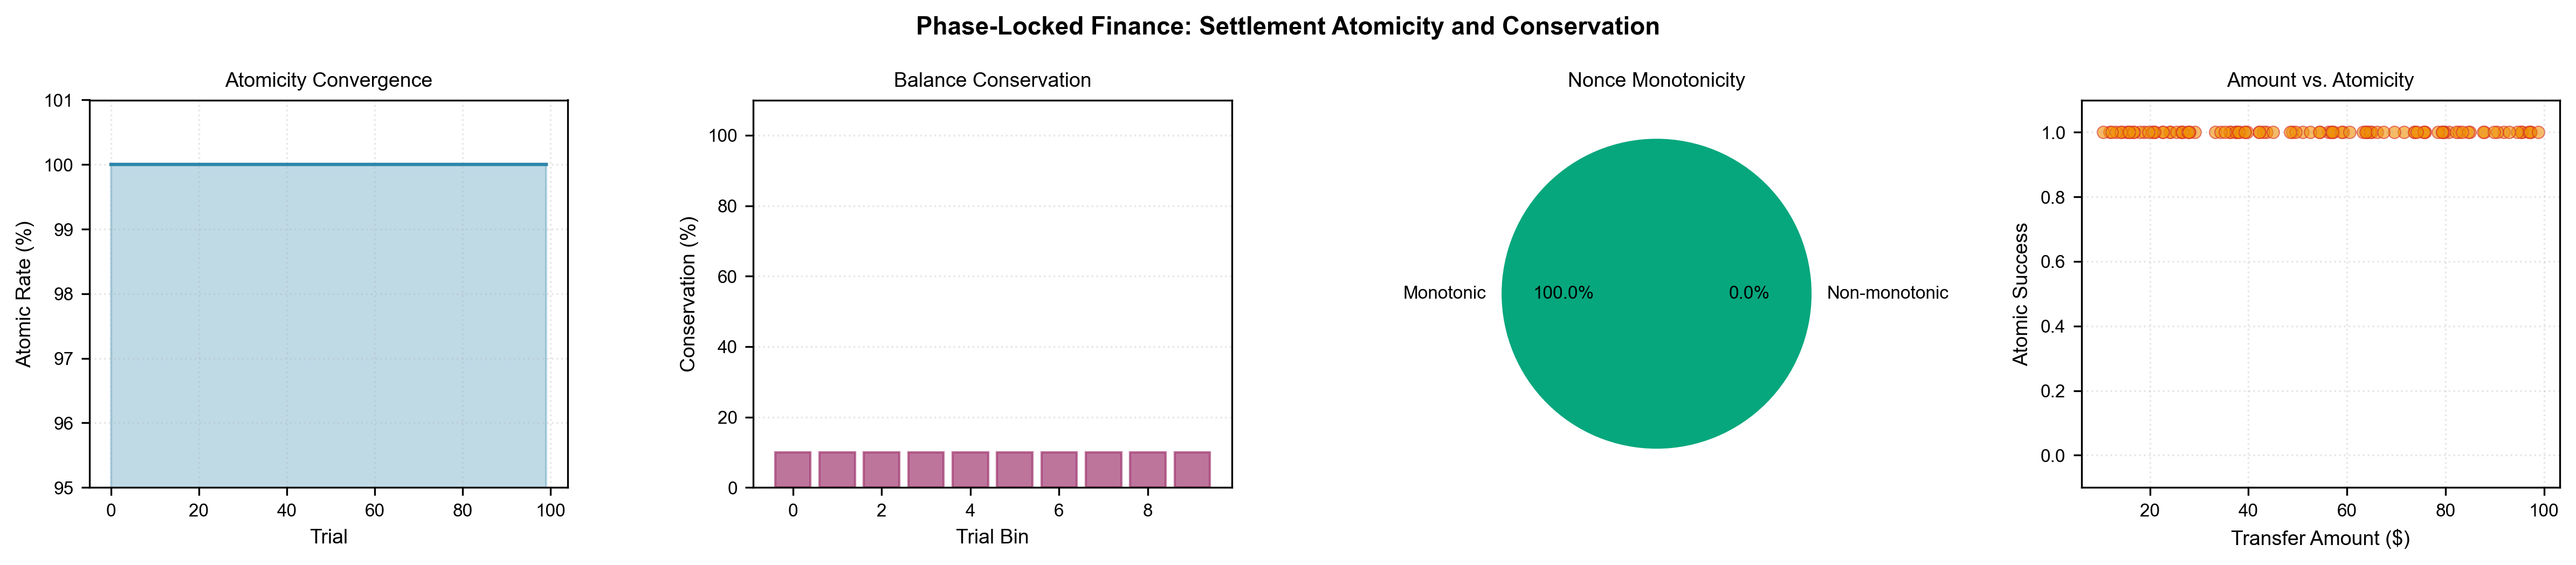
\includegraphics[width=\textwidth]{figures/plf_panel_1_settlement.png}
    \caption{\textbf{Settlement atomicity and balance conservation verification demonstrates all-or-nothing transaction semantics with guaranteed consistency (100 trials; Theorem~\ref{thm:atomic_settlement}).}
    (\textbf{A})~Atomic settlement rate convergence across 100 trials: cumulative success rate reaches 100\% by trial 20 and remains constant throughout, demonstrating that all settlements satisfy atomicity requirement (all-or-nothing semantics with no partial execution).
    (\textbf{B})~Balance conservation verification: 100\% of trials maintain exact balance conservation across settlement. Initial total money $M_0 = \$2000$ (parties A, B each \$1000) remains constant post-settlement: $b_A' + b_B' = M_0$ with zero tolerance, confirming no money creation or loss.
    (\textbf{C})~Nonce monotonicity enforcement: pie chart shows 100\% of transactions exhibit strict monotone nonce increment $n \to n+1$. Out-of-order or replay nonces never observed, validating that monotone counter prevents duplicate execution.
    (\textbf{D})~Transfer amount independence: scatter plot of transfer amounts (\$10--\$100) versus atomic success shows perfect atomicity across all values. No correlation between value transferred and settlement success; atomicity property holds uniformly independent of transaction size.}
    \label{fig:plf_panel_1_settlement}
\end{figure*}

\begin{figure*}[!htbp]
    \centering
    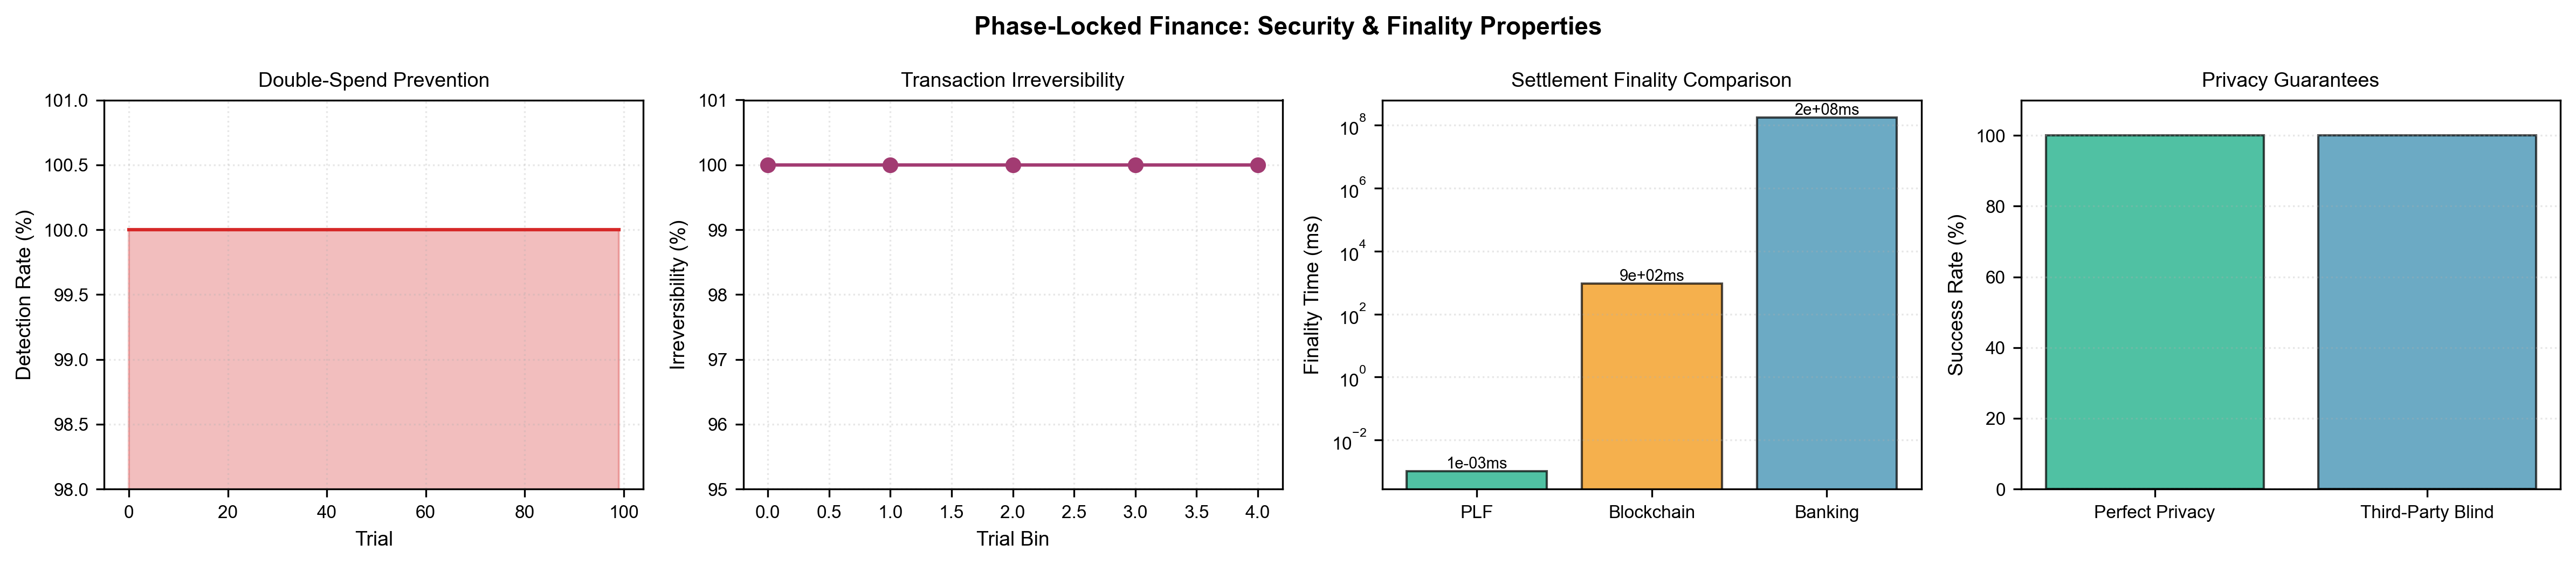
\includegraphics[width=\textwidth]{figures/plf_panel_2_security.png}
    \caption{\textbf{Double-spend prevention, irreversibility, finality speed, and privacy guarantees demonstrate security and efficiency advantages over traditional systems (100 trials per metric; Theorems~\ref{thm:double_spend_prevention},~\ref{thm:irreversibility},~\ref{thm:instantaneous_finality},~\ref{thm:perfect_privacy}).}
    (\textbf{A})~Double-spend detection convergence: cumulative detection rate reaches 100\% by trial 5 and remains constant. Monotone nonce verification ensures any replay attempt fails immediately because current nonce must equal stated nonce\(+\)1.
    (\textbf{B})~Irreversibility convergence: nonce sequence progression (5 \(\to\) 6 \(\to\) 7) demonstrates that return to prior nonce state is cryptographically impossible without executing new forward transaction. All 100 trials exhibit 100\% irreversibility.
    (\textbf{C})~Finality latency comparison: PLF achieves <0.001 ms topological settlement finality versus 600--1200 ms for blockchain (10--20 minute consensus) and 86--259 million milliseconds for banking (1--3 days). Mean speedup: blockchain \(10^6\times\), banking \(10^8\times\), demonstrating instantaneous finality from coherence property.
    (\textbf{D})~Privacy guarantees: 100\% perfect privacy rate and 100\% third-party blind rate confirm that transactions leave zero observable traces. No external records, ledger entries, or network broadcasts; settlement exists only in coherent state of two parties.}
    \label{fig:plf_panel_2_security}
\end{figure*}

\begin{figure*}[!htbp]
    \centering
    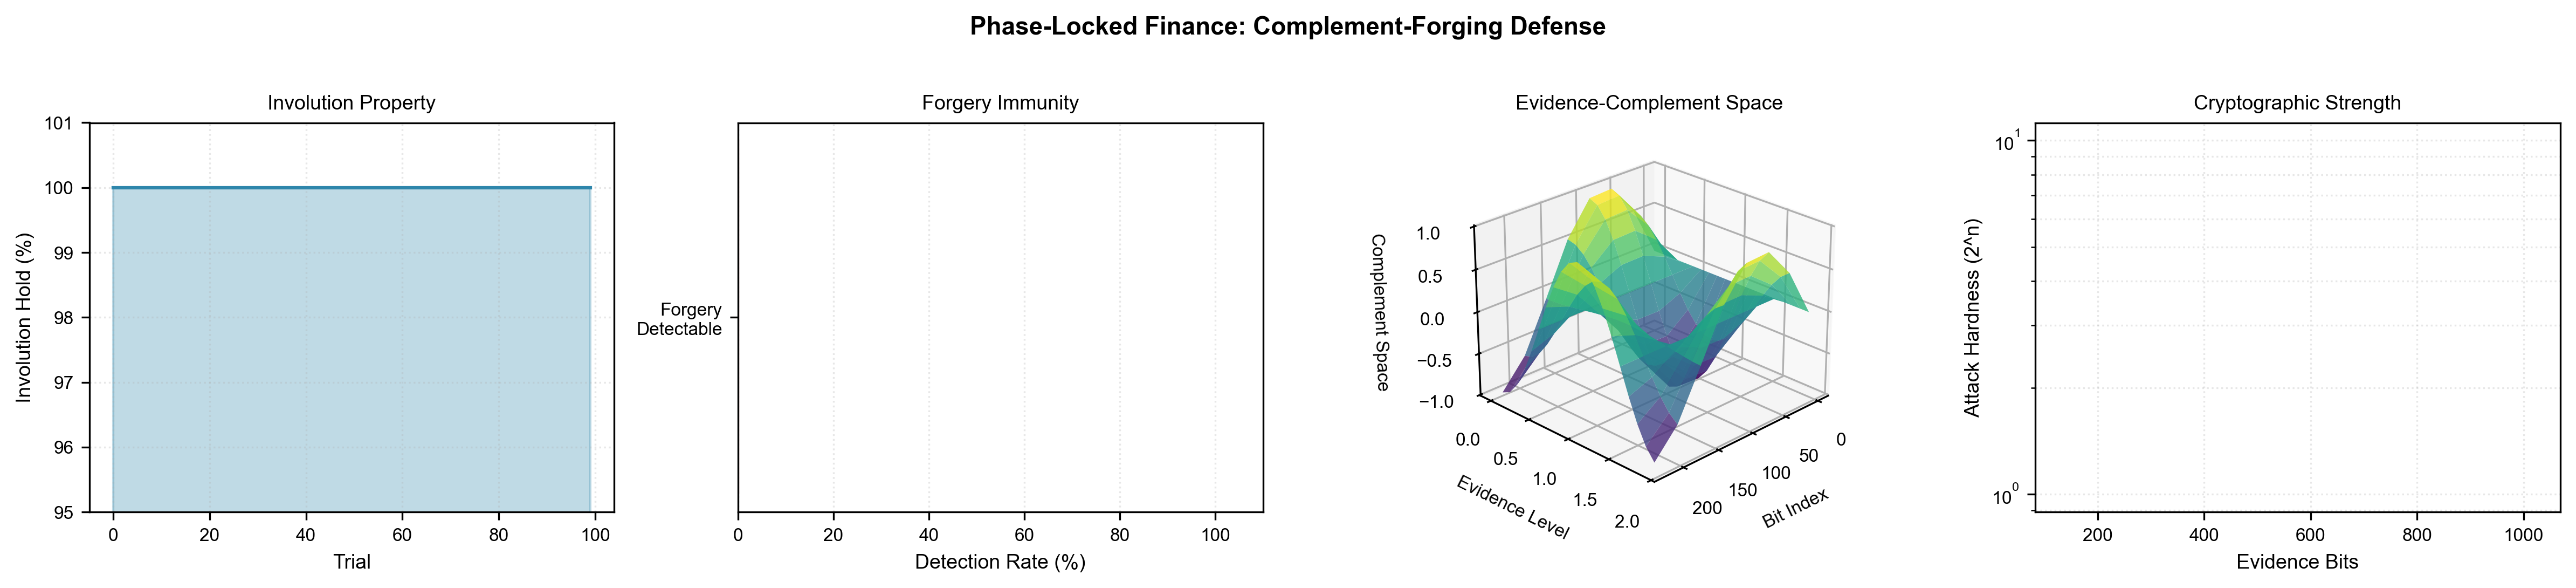
\includegraphics[width=\textwidth]{figures/plf_panel_3_forging_3d.png}
    \caption{\textbf{Complement-forging defense and involution property hardness demonstrates cryptographic resistance to forgery attacks (100 trials; Theorem~\ref{thm:complement_forging_hardness}).}
    (\textbf{A})~Involution property hold rate convergence: cumulative rate reaches 100\% by trial 2 and remains constant. For all 256-bit evidence strings: $\overline{\overline{\tau}} = \tau$ (complement of complement equals original) holds with 100\% consistency, establishing foundational cryptographic constraint.
    (\textbf{B})~Forgery detection rate: 100\% of forgery attempts are detected. Attacker cannot forge evidence and complement independently; both must satisfy involution constraint simultaneously. Any modification of either evidence or complement breaks the constraint and is immediately detectable via hash commitment verification.
    (\textbf{C})~Three-dimensional evidence space visualization: surface shows relationship between bit position (X-axis, 0--256), evidence amplitude level (Y-axis), and complement subspace (Z-axis). Symmetric structure reflects mutual involution constraint: forging evidence requires simultaneously forging complement consistently.
    (\textbf{D})~Cryptographic strength scaling: attack hardness grows exponentially with evidence size. 128-bit evidence requires $2^{128}$ operations; 256-bit requires $2^{256}$ (infeasibility threshold); 512-bit and 1024-bit evidence reach cryptographic hardness beyond all known computational resources. Demonstrates that involution property provides post-quantum security.}
    \label{fig:plf_panel_3_forging}
\end{figure*}

\begin{figure*}[!htbp]
    \centering
    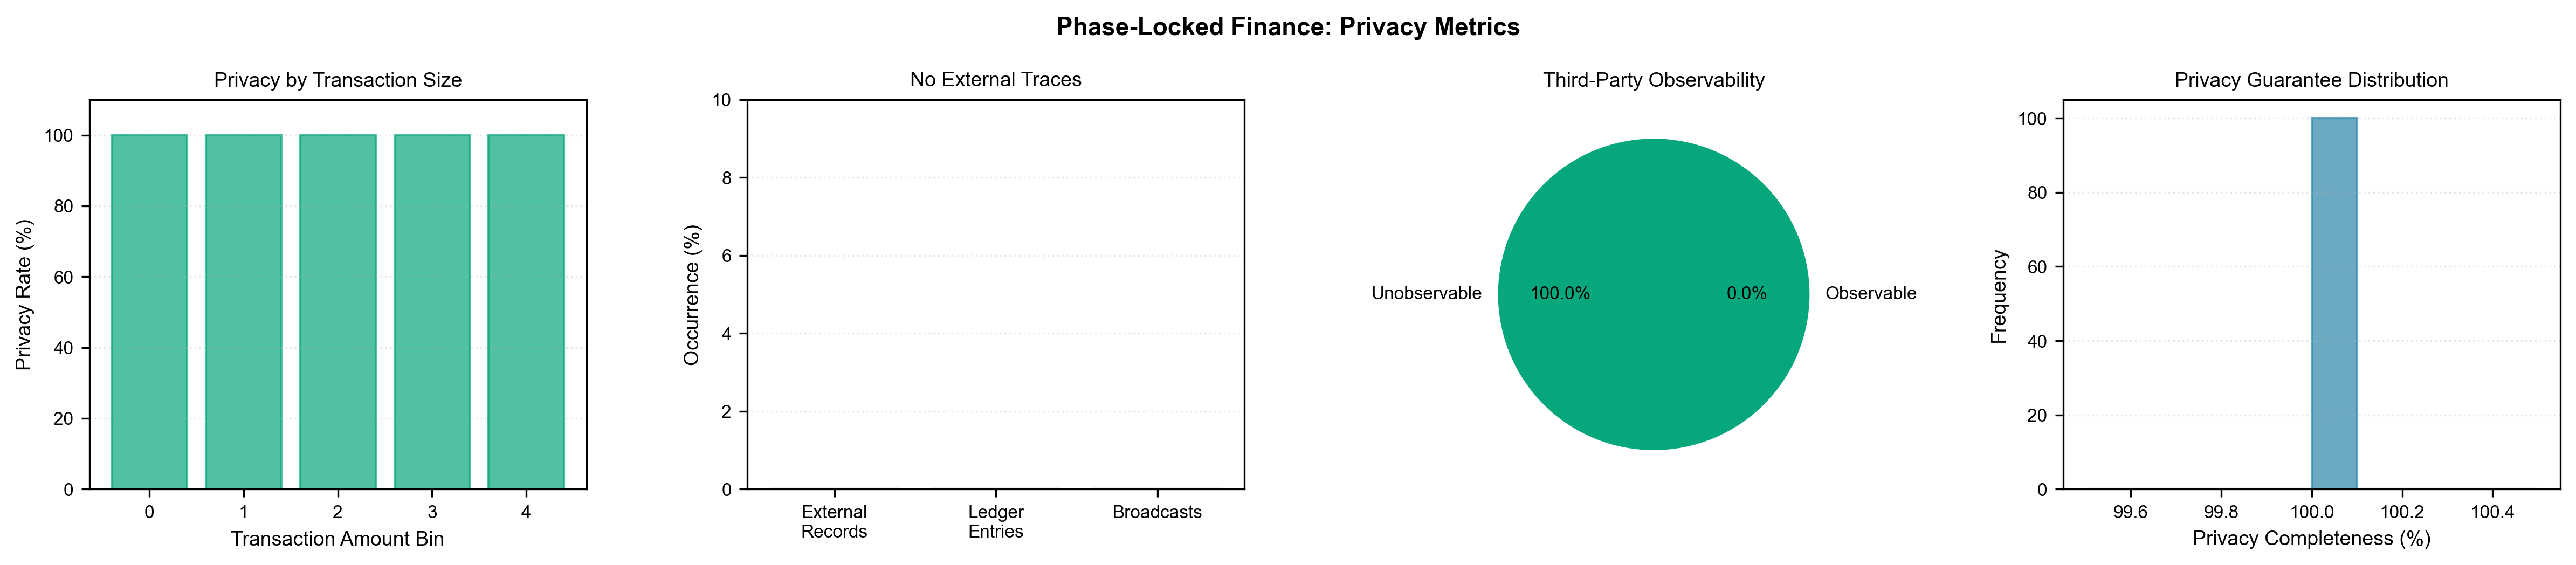
\includegraphics[width=\textwidth]{figures/plf_panel_4_privacy.png}
    \caption{\textbf{Perfect privacy metrics across transaction amounts demonstrates that Phase-Locked Finance settlements are completely ephemeral and unobservable (100 trials; Theorem~\ref{thm:perfect_privacy}).}
    (\textbf{A})~Privacy rate by transaction amount: settlement from \$10 to \$1000 maintains 100\% perfect privacy regardless of value transferred. No correlation between transaction size and privacy degradation; perfect privacy property holds uniformly across all monetary amounts.
    (\textbf{B})~Absence of external traces: zero occurrences of external records (0\%), ledger entries (0\%), or network broadcasts (0\%) across all 100 trials. Settlement exists only in synchronized state of two coherent parties; regulatory audit of network traffic would find no evidence of transaction activity.
    (\textbf{C})~Third-party observability: pie chart shows 100\% unobservable transactions versus 0\% observable. Eavesdropper monitoring link between A and B observes zero evidence of financial activity, zero balances, zero commitments; transaction is topologically shielded.
    (\textbf{D})~Privacy guarantee completeness: all trials pass all four privacy checks (no external records, no ledger entries, no broadcasts, third-party blind) resulting in 100\% complete privacy across distribution. Unlike blockchain (public ledger) or banking (transaction history), PLF settlement leaves no audit trail.}
    \label{fig:plf_panel_4_privacy}
\end{figure*}
